\section{Cyclic Groups}

\subsubsection*{Recall}
\begin{itemize}
    \item If $G$ is a group, $a \in G$, and $G = \{a^n : n \in \bb{Z}\}$ then $G = \struct{a}$ is a \itl{cyclic group} generated by $a$.
    \item Every cyclic group is Abelian.
    \item The \itl{Division Algorithm}: if $m \in \bb{Z}^+$ and $n \in \bb{Z}$, then there exists unique $q,r \in \bb{Z}$ such that
    \[
        n = mq + r \tand 0 \leq r < m.
    \]
\end{itemize}

\subsubsection{Thm. Cyclic Subgroups are Cyclic}
A subgroup of a cyclic group is cyclic.
\begin{proof}
    Let $G$ be a cyclic group, say $G = \struct{a}$, where $a \in G$. Let $H$ be a subgroup of $G$. Since $H \subseteq G$, every element of $H$ must be a power of $a$. Consider the \itl{smallest} positive power of $a$, $a^m \in H$, for $m \in \bb{Z}^+$. Let $a^n \in H \tfor n \in \bb{Z}$.

    By the division algorithm, there exists unique, $\exists! q,r \in \bb{Z}$ such that $n = mq+r$ where $0 \leq r < m$. Then,
    \begin{align*}
        a^n & = a^{mq+r} = a^{mq}a^r \\
        a^r & = a^{-mq}a^n = (a^m)^{-q}a^n
    \end{align*}
    Since we know that $a^m \in H$, we know that $(a^m)^{-q} \in H$. We also asserted that $a^n \in H$. Thus, we can conclude that $a^r \in H$. But $0 \leq r < m$, and $m$ is the \itl{smallest} positive integer such that $a^m \in H$. Thus $r = 0$. So,
    \begin{align*}
        n & = mq + 0 = mq \\
        a^n & = a^{mq}
    \end{align*}
    Thus every element of $H$ takes the form $(a^m)^q$, and $H$ is cyclic, with generator $\struct{a^m}$.
\end{proof}

\subsubsection{Def. Cyclic Group of Order n}
If $G$ is a cyclic group of \itl{order} $n$, then
\[
    G = \struct{a} = \underbrace{\{e = a^0, a^1, a^2, \ldots, a^{n-1}\}}_{n~\text{elements}} \tand a^n = e.
\]
We say the \itl{order of $a$ is $n$}, meaning $a^n = e$. Otherwise, the order of $a$ is infinite, and hence the order of $G$ is infinite.

\subsubsection{Thm. Cyclic Groups and the Integer}
Let $G = \struct{a}$.
\begin{enumerate}
    \item Every cyclic group of order $n$ is isomorphic to $\group{\bb{Z}_n,+_n}$.
    \item Every cyclic group of order infinity is isomorphic to $\group{\bb{Z}, +}$.
\end{enumerate}

\begin{proof}
    \begin{enumerate}
        \item Let $G = \struct{a}$ be a cyclic group of order $n$. Then
        \[
            G = \{e=a^0, a^1, a^2, \ldots, a^{n-1}\}
        \]
        Consider $\bb{Z}_n = \{0,1,2,\ldots,n-1\}$. Define $\phi: \bb{Z}_n \rightarrow G$ by $\phi(x) = a^x$.
        \begin{enumerate}
            \item One-to-one: assume $a^x = a^y$. Then $x=y$. Thus $\phi$ is one-to-one.
            \item Onto: let $a^x \in G$. Then choose $x \in \bb{Z}_n$, and $\phi(x) = a^x$. Thus, $\phi$ is onto.
            \item Operation Preserving: $\phi(x+y) = a^{x+y} = a^xa^y = \phi(x)\phi(y)$. Thus $\phi$ is operation preserving.
        \end{enumerate}
        Thus $\phi$ is an isomorphism and $\group{\bb{Z}_n,+_n} \simeq G$.
        \item Follows nearly identical as above.
    \end{enumerate}
\end{proof}

\subsubsection*{Note}
The above theorem implies that all cyclic groups of order $n$ are isomorphic to each other, and all cyclic groups of order infinity are isomorphic to each other. This is because isomorphism is an equivalence relation.

\subsection{Subgroups of Cyclic Groups}

\subsubsection{Thm. Order of Subgroups of Cyclic Groups}
Let $G = \struct{a}$ by a cyclic group of order $n$. Let $b \in G$ and let $b = a^s$ for $s \in \bb{Z}$. Then $\struct{b}$ is a cyclic subgroup of $G$ containing $\frac{n}{d}$ elements, where $d = \gcd(n,s)$.

\subsubsection{Cly. Order of Subgroups of Cyclic Groups}
If $G = \group{a}$ is a cyclic group of order $n$, then the other generators of $G$ are the elements of the form $a^r$ where $\gcd(n,r) = 1$.

\subsubsection*{Cyclic Subgroup Diagrams}
Example cyclic diagram for $\bb{Z}_{12} = \struct{Z}$.
\begin{center}
    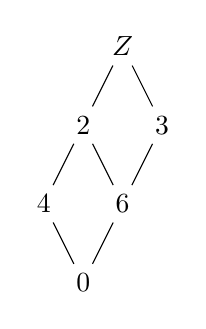
\begin{tikzpicture}
        \foreach \rank/\elements/\size in {1/{Z}/1, 2/{2,3}/2, 3/{4,6}/3, 4/{0}/2} {
        \foreach[count = \i] \element in \elements {\node (\element) at (\i - \size / 2, -\rank) {$\struct{\element}$};}
        }
        \foreach \j/\l in {Z/2, Z/3, 2/4, 2/6, 3/6, 4/0, 6/0} {\draw (\j) -- (\l);}
    \end{tikzpicture}
\end{center}

\subsection{Infinite Cyclic Groups}
The subgroups of $\group{\bb{Z},+}$ are of the form $\group{n\bb{Z}, +}$ for $n \in \bb{Z}$. For example,
\begin{align*}
    2\bb{Z} & = \{\ldots, -4,-2,0,2,4,\ldots\} \\
    5\bb{Z} & = \{\ldots, -10,-5,0,5,10,\ldots\}
\end{align*}